\chapter{The Solution}

This chapter will present EcoBeach, a highly resilient distributed system that can process satellite imagery in real-time and analyze the difference in water levels on given geo-locations.
EcoBeach collects data from beach locations (hence the name EcoBeach). Limiting geo locations to beaches in select countries is a deliberate choice, as the available server resources currently restrict the solution's scalability. \medbreak
\noindent
In \autoref{sec:solution-approach} \nameref{sec:solution-approach} EcoBeach will be described at a high-level. First, a summary of solutions to the sub-problems in \autoref{sec:problem-description} is given. Next, the infrastructure of EcoBeach is presented to show how the solutions to each of the sub-problems complement each other to provide a feasible solution to monitoring shorelines.

Lastly, the advantages and disadvantages of EcoBeach will be presented.

\section{Solution Approach}\label{sec:solution-approach}

EcoBeach consists of services and applications that play a crucial role in monitoring shorelines. There is a total of 11 services/applications as shown in \autoref{tab:ecobeach-services}.

\begin{table}[]
    \centering
    \begin{tabular}{| p{0.25\linewidth} | p{0.7\linewidth} |}
        \hline
        \textbf{Service name}      & \textbf{Service description}                                                                                                              \\ \hline
        Sentinel Satellite Scraper & A python script that downloads and pre-processes satellite imagery                                                                        \\\hline
        NDWI Analyzer              & A Spark job that analyzes pre-processed satellite images for shoreline changes.                                                           \\\hline
        Kafka                      & A distributed event streaming service, where intermediary data is saved as part of the processing pipeline.                               \\\hline
        Spark                      & A large-scale data analytics framework that supports publishing jobs that are processed on distributed Spark Workers.                     \\\hline
        Hadoop                     & A framework that allows distributed file storage primarily with HDFS. Used for saving checkpoints and the pre-processed satellite images. \\\hline
        Zookeeper                  & A centralized service to enable reliable distributed coordination for Hadoop and Kafka.                                                   \\\hline
        MongoDB                    & A distributed database to save and query fully processed data.                                                                            \\\hline
        MongoDB Kafka Connector    & A sink connector for Kafka to feed fully processed data from Kafka to MongoDB                                                             \\\hline
        Kowl                       & An intuitive monitoring service that allows viewing and configuring running Kafka services.                                               \\\hline
        WebAPI                     & A .NET WebAPI to provide a nice interface for querying data from MongoDB                                                                  \\\hline
        Android Application        & The EcoBeach app where fully processed data is represented with the google maps interface.                                                \\\hline
    \end{tabular}
    \caption{The services/applications in the EcoBeach system}
    \label{tab:ecobeach-services}
\end{table}

\noindent
The services in EcoBeach were chosen or created to provide solutions to the sub-problems. Below a summary of each solution to the sub-problems is presented.

\paragraph{How to download satellite images from Copernicus?} To download satellite images, we created a resilient scraping service that continuously downloads and pre-processes satellite images on given geo-locations. The scraping service is described in detail in \autoref{subsec:sentinel-satellite-scraper}.

\paragraph{How to process images so water is differentiated from land?} For this purpose, we pre-process images during the scraping process, so they are saved as black and white images according to their \acrfull{ndwi} value. Then we created the NDWI Analyzer, a Spark Job, that analyzes downloaded satellite images to determine what is water or land. The NDWI Analyzer is described in \autoref{subsec:ndwi-analyzer}.

\paragraph{How to build a system capable of handling big data?} To create a system capable of large-scale data processing and analysis, we created a stack that relies on distributed systems that are very scalable and fault-tolerant. The stack includes Kafka, Spark, Hadoop, Zookeeper, and MongoDB and is described in \autoref{subsec:the-stack}

\paragraph{How to build a system capable of real-time processing?} The main contributor to this is Kafka and Spark. Kafka allows us to create topics with intermediary data, where our NDWI Analyzer Spark Job is set up as a consumer that processes new entries as they are created. Together with the rest of the stack, it allows us to create, process, and feed data to MongoDB quickly and reliably as new data is entering the system.

\paragraph{How to build a highly resilient system?} To make EcoBeach a resilient system, we identified single-points of failure and added load-balancing and distribution of services to ensure that the system would function reliably in case of failures. Docker Swarm as the chosen container orchestration tool was a massive help in configuring this. This is described in more detail in \autoref{subsec:the-infrastructure}.

\paragraph{How to build a mobile application that uses mobile sensing in a meaningful way to visualize shoreline changes?} To make the EcoBeach app utilize mobile sensing, we made the app rely on the user's current location and provide data accordingly. As the EcoBeach app is an Android application, the Google Maps API is what the app relies on to provide most of its features. The EcoBeach app is described in detail in \autoref{subsec:ecobeach-app}

\subsection{The infrastruture}\label{subsec:the-infrastructure}
- Present the infrastructure diagram
- Explain the infrastructure diagram
- dont go in depth here, thats what we have the Hosting Setup for.

\subsection{Advantages and disadvantages of EcoBeach}
- Advantages of the solution
- Disadvantages of the solution

\section{Solution Description}

In this section, an in-depth description of the solution is presented. First, the hosting setup and the central services that drive the data pipeline are explained. After this, the services that create, read, process, and visualize data in EcoBeach are presented.

\subsection{HDFS, Kafka, Spark and MongoDb} \label{subsec:the-stack}

– Purpose (Why?)
– Context (When?)
– Description (How?)

- Distributed File System
- Distributed Event Streaming
- Large-scale data analytics
- Distributed Database

\subsection{Sentinel Satellite Scraper}\label{subsec:sentinel-satellite-scraper}
The \acrfull{sss} is a python script created to scrape and continuously download satellite imagery from given geo-locations. The script was created as EcoBeach relies on the analysis of geo-locations to determine how shorelines are changing. Because of this, it requires a steady input of data to reliable show how shorelines historically and currently have changed.\\\\
\noindent
The \acrshort{sss} runs every week to scrape satellite images for beaches in Denmark, Sweden, Germany, and Great Britain. Each subsequent run scrapes imagery three years back from the current date. It only downloads images that the EcoBeach pipeline has not previously processed by caching completed work. Subsequent runs are much faster due to this caching strategy. \\\\
\noindent
To understand the intricacies of the \acrshort{sss}, one must understand the format of the data downloaded from the Sentinel Satellite. It is essential to mention the script downloads satellite imagery from the Sentinel-2 satellite.

\subsubsection{Sentinel-2 satellite data products}

The Sentinel-2 satellite has two types of products available for download. The two product types are Level-1C and Level-2A as illustrated in \autoref{tab:sentinel-2-product-types}.

\begin{table}[h!]
    \centering
    \begin{tabular}{| p{0.15\linewidth} | p{0.35\linewidth} | p{0.35\linewidth} |p{0.15\linewidth} |}
        \hline
        \textbf{Product name} & \textbf{High-level Description} & \textbf{Data Volume} \\ \hline
        Level-1C              & Top-of-atmosphere               & 600MB — 100x100 km2  \\\hline
        Level-2A              & Bottom-of-atmosphere            & 800MB — 100x100 km2  \\\hline
    \end{tabular}
    \caption{Adapted from \href{https://sentinels.copernicus.eu/web/sentinel/missions/sentinel-2/data-products}{Sentinel-2 data products}}
    \label{tab:sentinel-2-product-types}
\end{table}

EcoBeach relies on Level-2A products, as these are ground images and not atmospheric images. The Level-2A products can be downloaded in 3 different spatial resolutions, 10m, 20m, 60m, all as tiles covering 100x100 $km^2$. The spatial resolution defines how many cubic meters each pixel covers and what spectral bands are available. Naturally, the lower the spatial resolution is, the more detailed the product is. However, it also increases its size to $\sim 1GB$ per product at 10m spatial resolution. \\

As previously mentioned, each spatial resolution contains different spectral bands. The 10m spectral resolution is the one the \acrshort{sss} uses, and it includes four spectral bands: band 2, band 3, band 4, and band 8, which defines the different wavelengths the Sentinel-2 Satellite can capture. The specifications of these bands can be seen in \autoref{tab:sentinel-2-10m-bands}.
\cite{sentinel-2-product-specification}

\begin{table}[h!]
    \centering
    \begin{tabular}{| p{0.1\linewidth} | p{0.3\linewidth} | p{0.3\linewidth} | p{0.3\linewidth} |}
        \hline
        \textbf{Band} & \textbf{Central wavelength} & \textbf{Color}                   \\ \hline
        B2            & 496.6 nm                    & Blue                             \\ \hline
        B3            & 560.0 nm                    & Green                            \\ \hline
        B4            & 664.5 nm                    & Red                              \\ \hline
        B8            & 836.1 nm                    & Visible and Near Infrared (VNIR) \\ \hline
    \end{tabular}
    \caption{Adapted from \href{https://sentinels.copernicus.eu/web/sentinel/missions/sentinel-2/data-products}{Sentinel-2 data products}}
    \label{tab:sentinel-2-10m-bands}
\end{table}

\subsubsection{The implementation and design}

\acrshort{sss} uses quite a few python libraries to download products, combine bands, pre-processing, and produce Kafka messages. The first and arguably the most important is the \emph{sentinelloader} library. The \emph{sentinelloader} library is in control of the logic related to downloading the products from Sentinel-2, combining bands, and cropping the resulting image to the location of interest. Lets first have a look at the entry point of the script the \emph{scrape(args)} method in \autoref{fig:sentinel-satellite-scraper-scrape}.

\begin{figure}[h!]
    \centering
    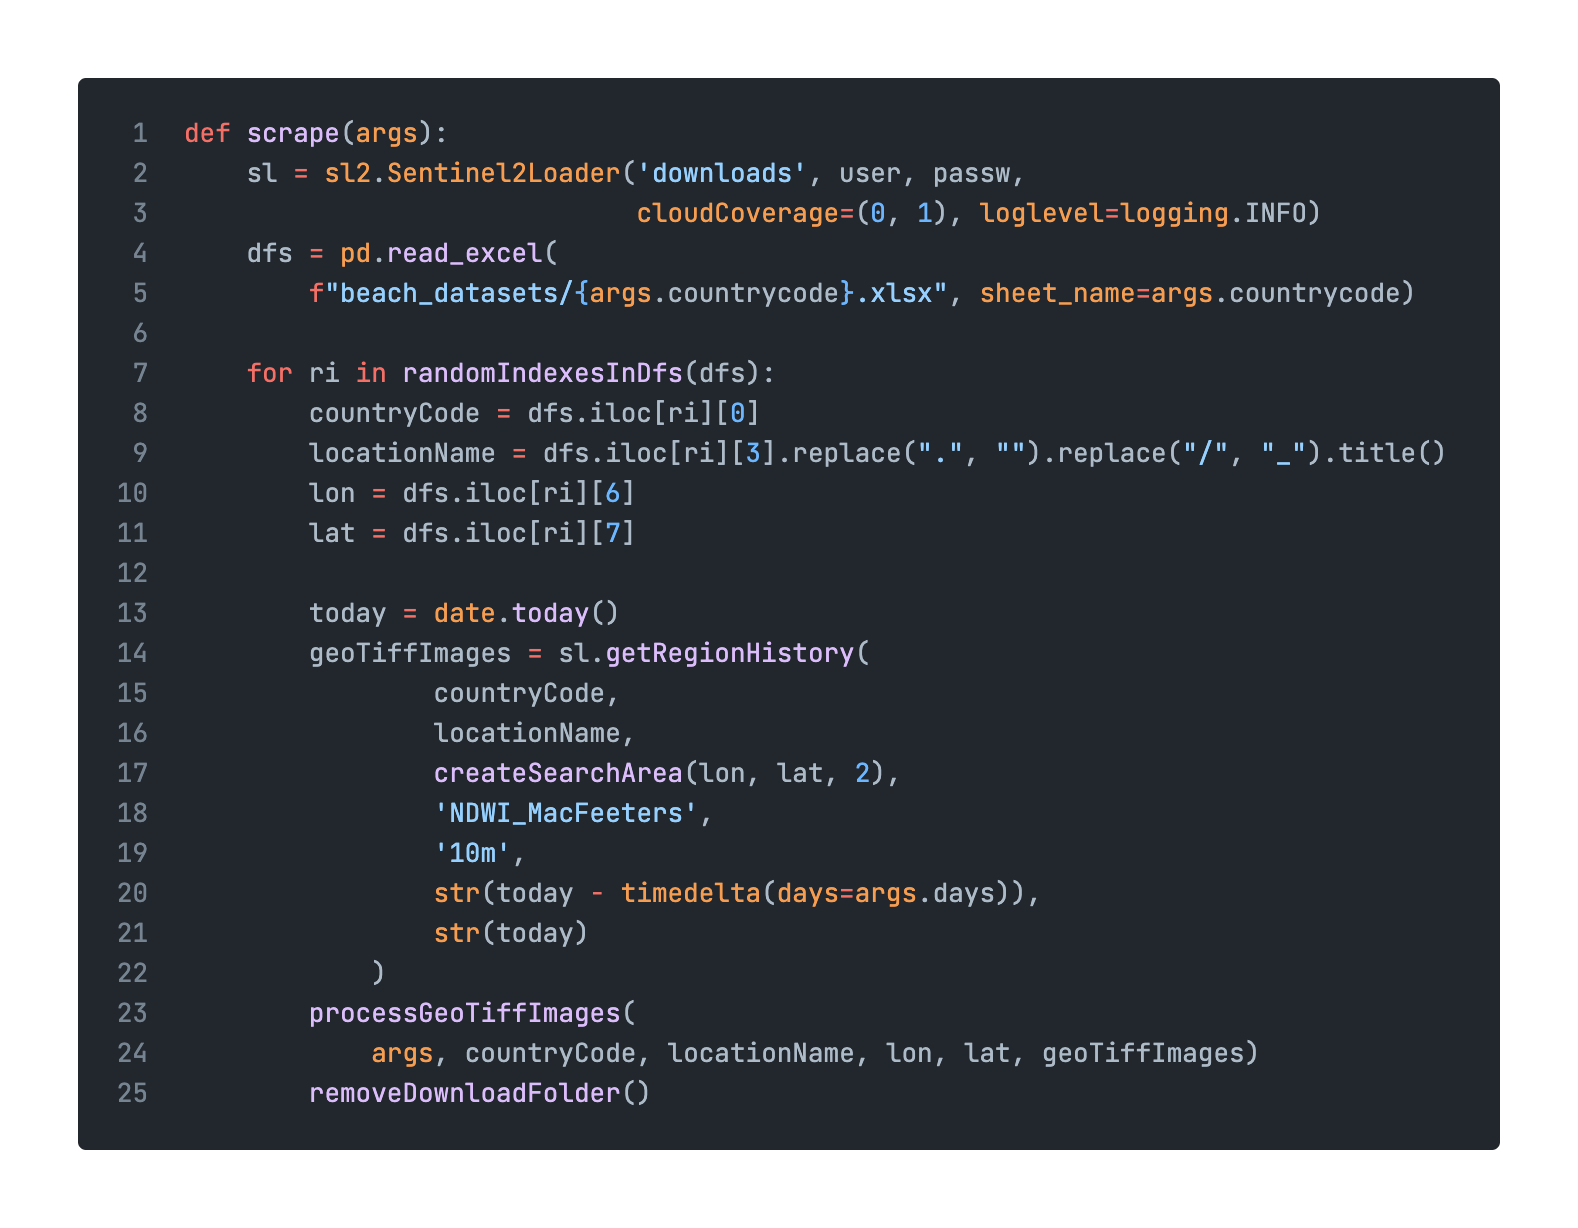
\includegraphics[width=\textwidth]{sentinel-satellite-scraper-scrape.png}
    \caption{The \emph{scrape(args)} methodh that is the entry point of the \acrshort{sss}.}
    \label{fig:sentinel-satellite-scraper-scrape}
\end{figure}

The scraping method first instantiates the \emph{Sentinel2Loader} from the \emph{sentinelloader} library with the folder to download products too, the Copernicus user, the desired cloud coverage percentage, and the log level. After initialisation the locations to scrape for are read in from one of many excel files located in the scrapers directory. Each of these Excel files contains geo-locations on beaches in a specific country and come from a publicly available dataset from the European Environmental Agency \cite{bathing_dateset}. 

When the Excel data has been read to memory, the main scraping loop begins, where it randomly selects a non-processed beach and proceeds. Randomly selecting a beach is a deliberate choice as the Copernicus API restricts the number of offline products that can be downloaded to 20 each day. Mixing up which locations we query historical data from ensures we use the offline product retrievals differently each time the script is run. Thus, we improve the chances of getting historical data for different areas over time.

Next, the different needed parameters are extracted from the excel data, and the process of downloading products, combining bands, and cropping the resulting images is started by the \emph{getRegionHistory(...)} method call. This call is called with the country code, the location name, a search area that defines the boundary of the location of interest, the index we want to combine bands, the spatial resolution, the from date, and lastly, the to date.

As indicated by the ``NDWI\_MacFeeters`` parameter, the combination of bands happens accordingly to the \acrfull{ndwi} \cite{ndwi}. The MacFeeters formula for \acrshort{ndwi} combines the bands into an image that differentiates water from land. The \acrshort{ndwi} uses a simple formula to combine band 3 and band 8 to give a value between 0 and 1 for each pixel that indicates how likely that pixel is to be either water or land. \cite{sentinel-2-bands-combinations}

\[ NDWI = \dfrac{B3 - B8}{B3 + B8} \]

Furthermore, the cropping of the image relies on the provided search area that defines the boundaries of the location of interest. \emph{Sentinelloader} automatically crops out the area of interest from the downloaded product(s). In cases where the place of interest covers multiple products, the \emph{sentinelloader} library can download, combine and crop the image from various products, so no data is lost.

After having downloaded products, combined bands, and cropped the resulting image, custom pre-processing is done on the resulting image to color it based on the \acrshort{ndwi} values and to ensure the image size is as compact as possible. This work happens in the \emph{processGeoTiffImages(...)}.

\begin{figure}[h!]
    \centering
    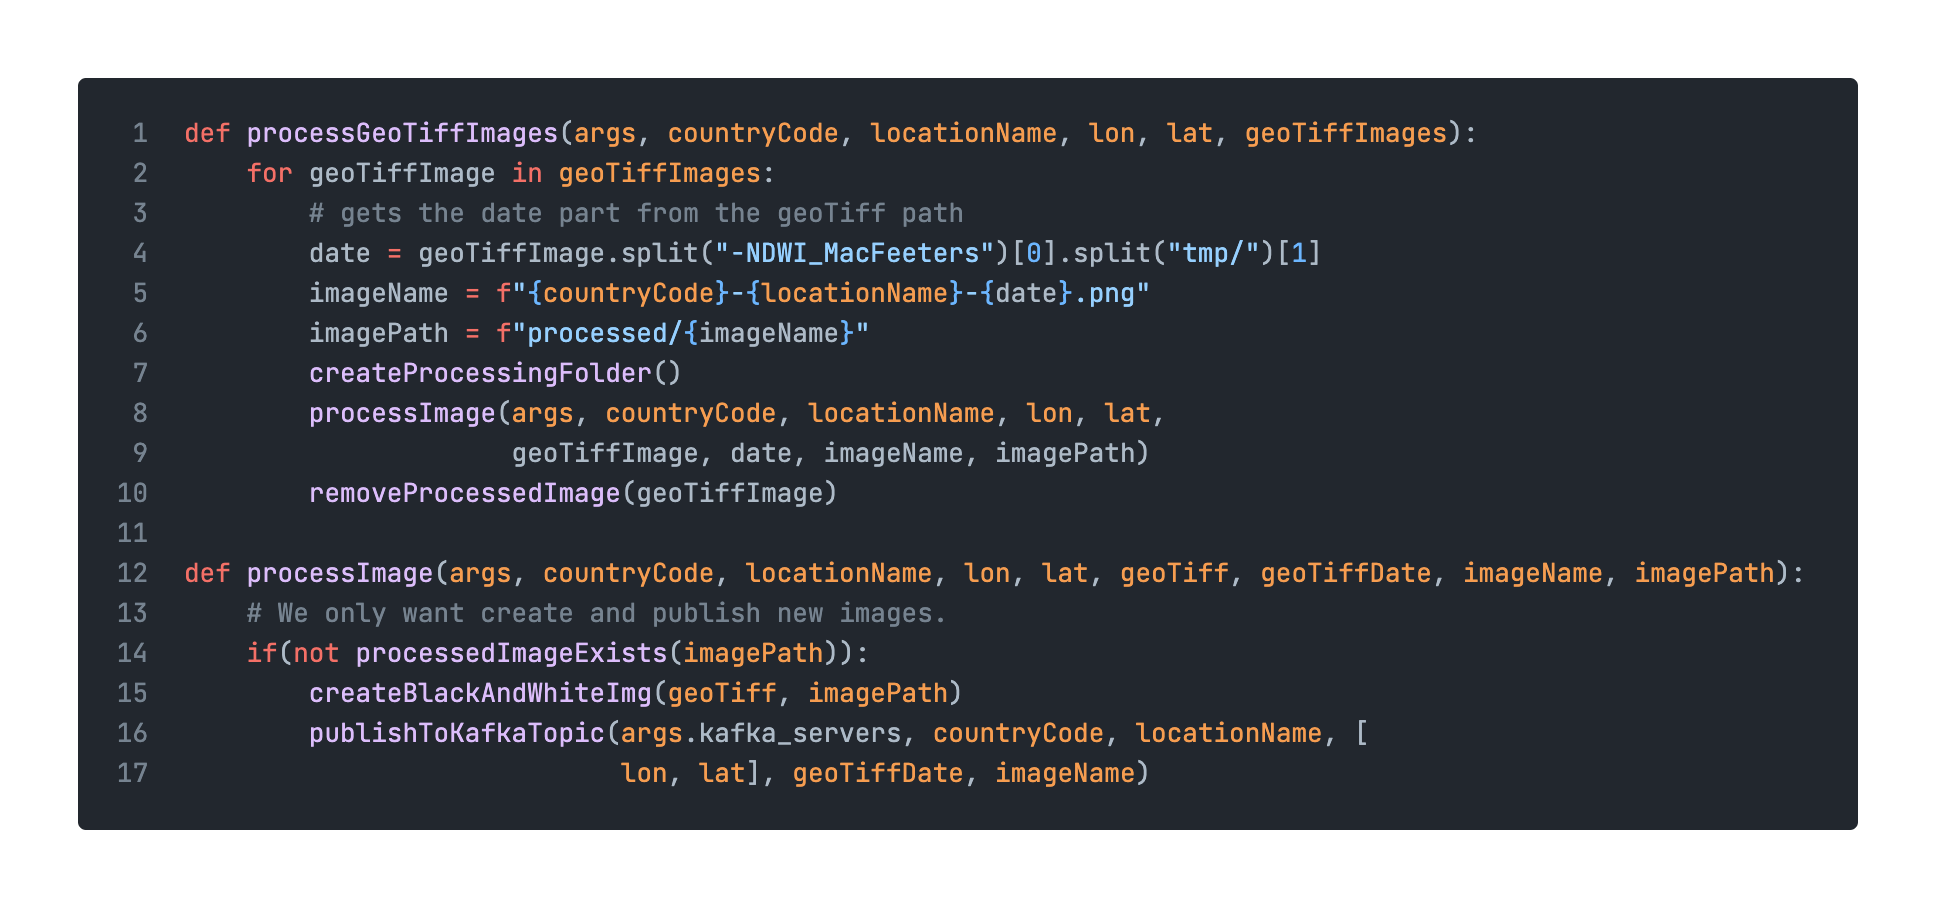
\includegraphics[width=\textwidth]{sentinel-satellite-scraper-pre-processing.png}
    \caption{The \emph{scrape(args)} method that is the entry point of the \acrshort{sss}.}
    \label{fig:sentinel-satellite-scraper-pre-processing}
\end{figure}

First, the desired image name and path of the pre-processed images are constructed from the downloaded images from the \emph{sentinelloader}. Then the downloaded images are passed on to the \emph{processImage(...)} method that first creates a new image from one of the downloaded images. The new image is combined with a black and white color map that paints any pixel with an \acrshort{ndwi} value greater than 0.6 white, and any pixel with an \acrshort{ndwi} value smaller than 0.6 black. Two of these images can be seen in \autoref{fig:sentinel-satellite-scraper-processed-image}.

\begin{figure}[h!]
    \centering
    \fbox{
\includegraphics[width=0.4\textwidth]{DK-EJERSLEVLYNG-2021-10-13.png}}
    \fbox{
\includegraphics[width=0.4\textwidth]{DK-GLSTRANDSKOV-2021-09-08.png}}
    \caption{Processed images of Ejerslevlyng (left) and Gl Strandskov (right) beaches in DK with the black and white colormap applied.}
    \label{fig:sentinel-satellite-scraper-processed-image}
\end{figure}

Finally, the image and relevant metadata are compressed to JSON and published to Kafka. After this, all downloaded satellite imagery is deleted to clear up valuable space for processing the following location. If this cleanup process is skipped, the downloaded products would quickly fill up the remaining disk space on the machines where the script is run.

\subsection{NDWI Analyzer}\label{subsec:ndwi-analyzer}

The NDWI Analyzer is a python spark job created to continuously consume and analyze messages from Kafka to provide insight into what the scraped satellite images can tell us about the water content changes. EcoBeach relies on distributed Spark workers to handle this job, to efficiently analyze newly scraped satellite images, and feed the results back to Kafka.\\\\
\noindent
The NDWI Analyzer runs constantly and watches for changes to the Kafka topic ``ndwi\_images``. Whenever a new message is added to the topic, the NDWI Analyzer consumes this message, analyzes it, and produces a new message to the ``ndwi\_results`` topic that holds all data that the data pipeline has fully processed.\\\\
\noindent
The analysis is a three-step process. First the black and white images in \autoref{fig:sentinel-satellite-scraper-processed-image} that are created by the \acrshort{sss} are recreated. The images are stored in the Kafka message that contains the image encrypted as byte64. Then all white and black pixels are counted in the image, and lastly, the percentage and area (in cubic meters) of both white (water) and black (land) pixels are calculated. The relevant code is shown in \autoref{fig:ndwi-analyzer-code}.

\begin{figure}[h!]
    \centering
    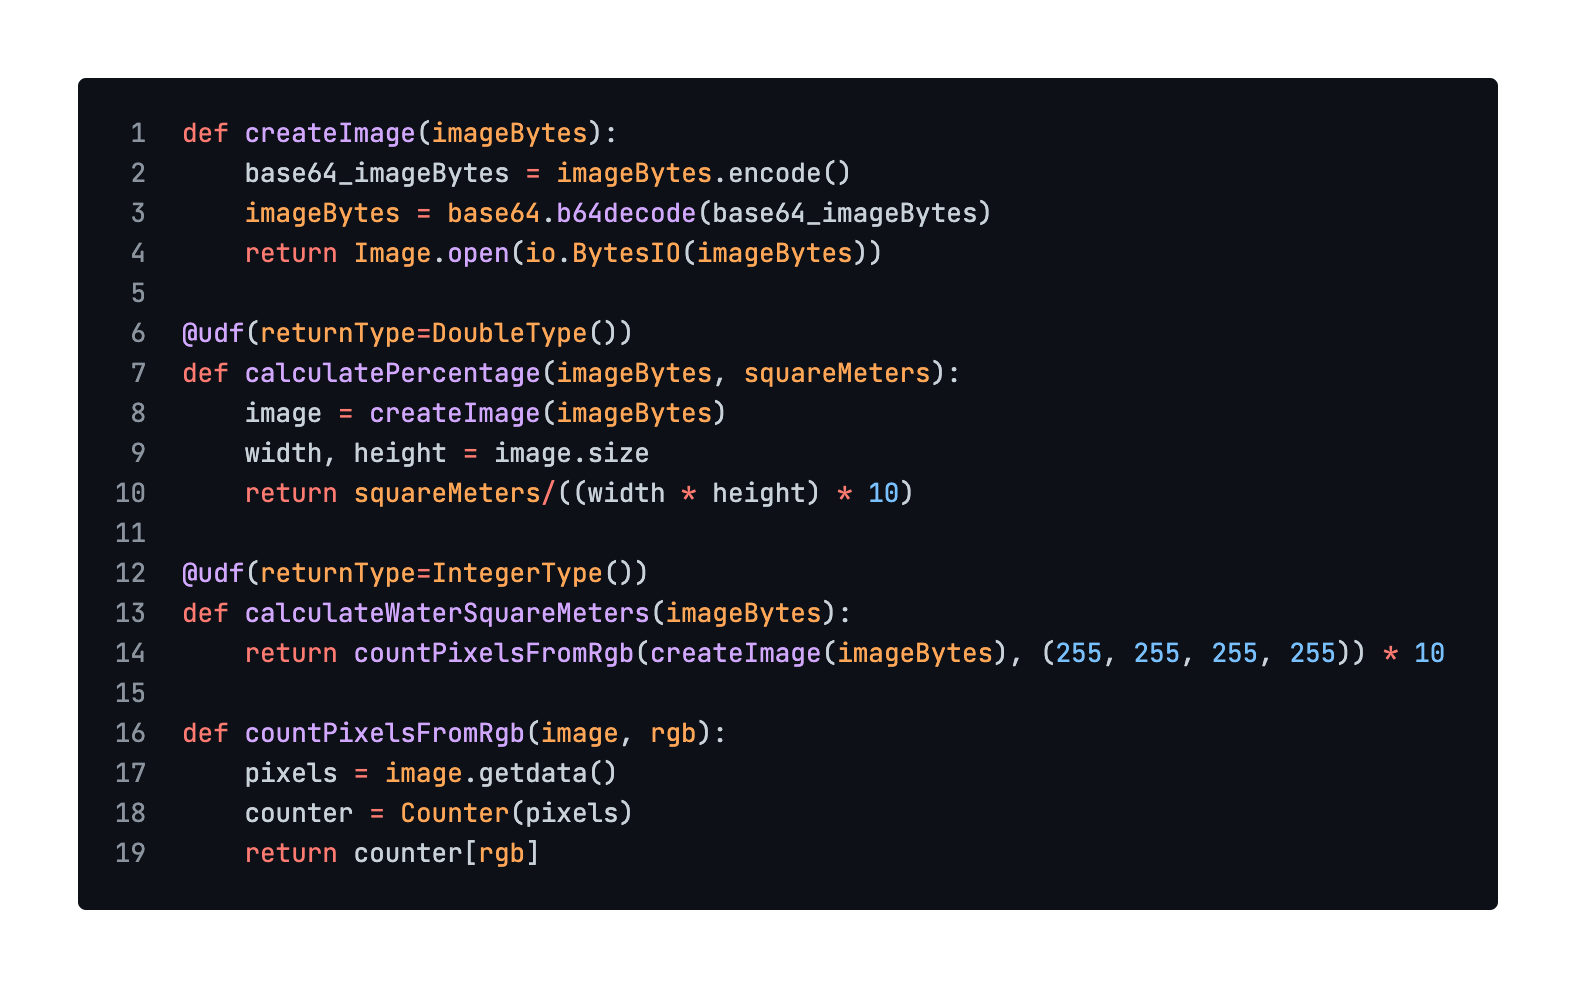
\includegraphics[width=\textwidth]{ndwi-analyzer-code.png}
    \caption{The code that recreates the black-and-white images, counts pixels and calculates percentage and area (in cubic meters) of water and land.}
    \label{fig:ndwi-analyzer-code}
\end{figure}

\subsection{WebAPI}

\subsection{EcoBeach App}\label{subsec:ecobeach-app}





